\documentclass[letterpaper,twocolumn,10pt]{article}
\usepackage{usenix2019_v3}

\usepackage{tikz}
\usepackage{amsmath}
\usepackage{paralist}
\usepackage{dblfloatfix}
\usepackage{fixltx2e}
\usepackage{caption}

\begin{document}
\date{}

\title{\Large \bf Reducing Compaction Process of LSM with LvlupDB}

\author{
    {\rm Jinghuan\ YU}\\
    Your Institution
    \and
    {\rm Second Name}\\
    Second Institution
} % end author

\maketitle

\begin{abstract}
    abstract abstract abstract abstract abstract abstract abstract abstract abstract abstract abstract abstract abstract abstract abstract abstract abstract abstract abstract abstract abstract abstract abstract abstract abstract abstract abstract abstract abstract abstract abstract abstract abstract abstract abstract abstract abstract abstract abstract abstract abstract abstract abstract abstract abstract abstract abstract abstract abstract abstract abstract abstract abstract abstract abstract abstract abstract
\end{abstract}

\section{Introduction}

With the development of big data technology, the volume and the throughput of modern application system has greatly increased. To improve writing performance of the application system, Google proposed Bigtable~\cite{chang2008bigtable} storage system in 2008 and introduce the great advantage of LSM data structure. Log Structured Merge Tree, also known as LSM~\cite{LSM_ori}, is a specially designed data structure optimizing warm writing performance proposed in 1996. Due to its high writing performance and simple index structure, LSM gets widely used in big data storage systems, in-memory databases and embedding databases like Hbase~\cite{ApacheHB8:online}, Cassandra~\cite{ApacheCa91:online},MongoDB~\cite{MongoDBD83:online}, LevelDB and SQLite. LSM uses the in-memory buffer to achieve high writing performance, it aggregates a batch of writing operations and flashes them into the storage system once the memory space is limited. This buffer and batch technique force the writing operations into sequential access to the file system. Although LSM can take advantage of more efficient read and write on the file system, it also introduces the compaction process to keep the entire order of the persistent record. This additional software-level overhead can cause significant performance jitters and write amplification.

\begin{figure}
    \begin{center}
        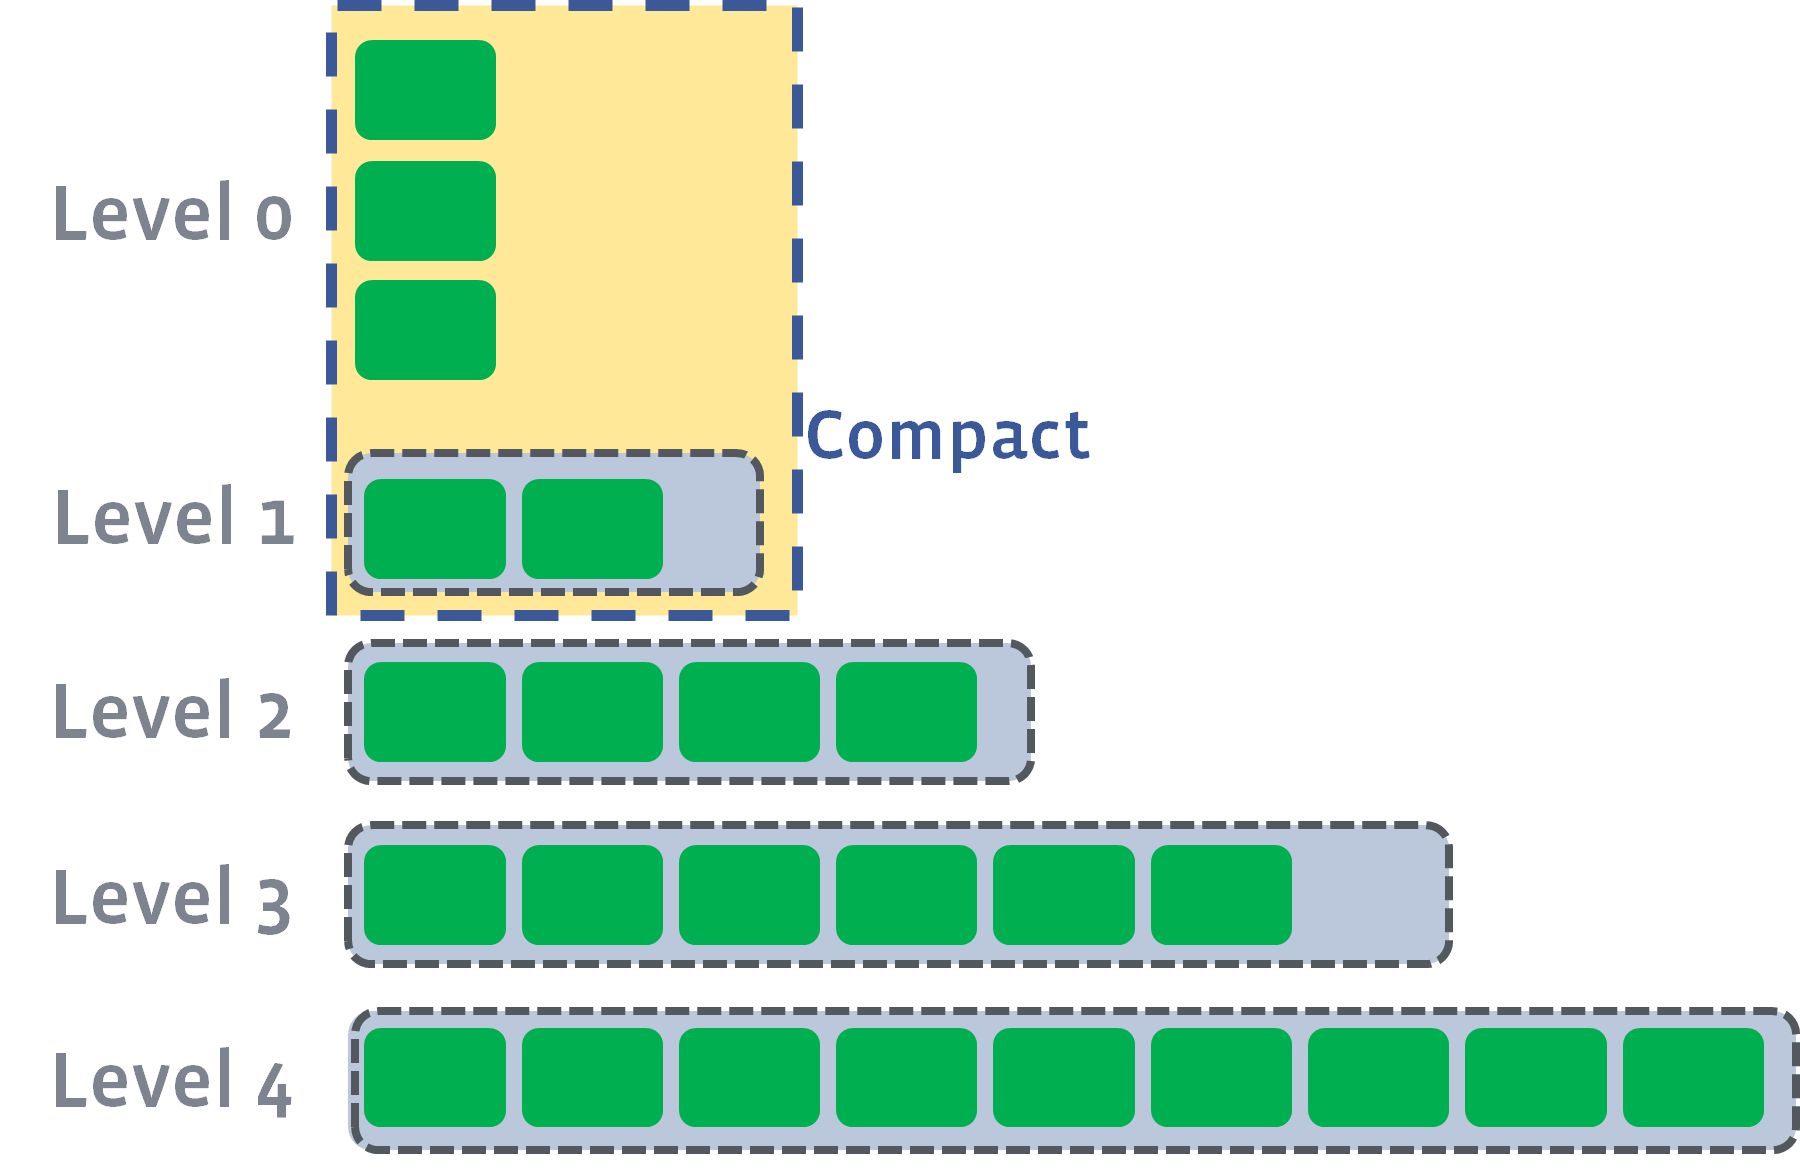
\includegraphics[width=\columnwidth]{2018-12-24-15-28-12.png}
    \end{center}
    \caption{\label{fig:simple_compaction} A typical compaction process starts with choosing the files need compaction most. Then the system will decode the persistent data into memory processing format and merge all the entries inside these files. At last, create a new file to store the processed entries and remove outdated files. It can be concluded as three main steps: 1. file choosing step; 2. entry merging step; 3. write out step.}
\end{figure}

There are two basic resources while analyzing the performance and bottleneck of a storage system:
\begin{inparaenum}[1)]
    \item the computation resources; and
    \item the data transmission resources referred to as I/O $(Input/Output)$ resources;
\end{inparaenum}
The Figure \ref{fig:simple_compaction} shows the basic steps of compaction process, unlike other operations in LSM-based system, most of processing in compaction will consume both two resources, especially the entry merging step. In merging step, the system firstly read a period of data from sorted string tables $(SST)$, decode it from the file format into in-memory format, then compare it with other entries.

There are many recent proposals focus on reducing the impact of compaction and improving throughput by using new storage materials~\cite{kannan2018redesigning,chen2017kvftl,zhang2017flashkv,xia2017hikv,wu2018kvssd,sun2018co,shen2017didacache}. Byte-addressed and fast nonvolatile memory such as 3D Xpoint~\cite{3dxpoint} can bring following priorities:
\begin{inparaenum}[1)]
    \item higher random access performance;
    \item lower in-place update latency; and
    \item better application-level parallelism.
\end{inparaenum}
With optimized redesigning of LSM structure~\cite{kannan2018redesigning}, the system can achieve higher throughput; combining with the improvements of its storage architecture and specific compaction algorithm of LSM can reduce the performance impact. Following this though, this paper proposes the idea of splitting specific level of SST files into persistent environment to reduce the total count of compactions during a period of time under a reasonable workload.

% this part starts the contribution part
This paper proposes the LvlupDB, focuses on the following problems. First, as the first level of SST files, level-0 files are produced by memtable directly, this means there can be many overlapping keys between these files. This makes several optimized compaction algorithm like parallel compaction and universal compaction~\cite{comapction_types,dayan2017monkey}. Moreover, this also causes additional overhead while processing this level, including picking more SST files, more complicated merging process. Second, typical LSM based system like LevelDB~\cite{LevelDBo14} only allows append only modification. Proposals\cite{kannan2018redesigning} advise in-place update approaches to take advantage of nonvolatile memory's  byte addressed feature and reducing the write amplification. But this still can not avoid performance impact caused by resource competition between workload and compaction process. The final problem, moving SST files hierarchically\cite{} or using NVM as cache~\cite{NVMRocks} will bring more cross access reading latency and use 


\section{Background}


\section{Motivation}

\section{Design}

\section{Evaluation}

\section{Related Work}

\section{Acknowledgements}


\bibliographystyle{plain}
\bibliography{lvlup.bib}


\end{document}
